% This nuaa-JUB.tex is a latex-beamer template using the JUB beamer theme produced by Billy Okal.
% URL: https://github.com/makokal/beamer-themes/tree/master/JUB
% 
% Copyright (c) 2011-2014, Billy Okal All rights reserved.
% 
% Redistribution and use in source and binary forms, with or without modification, are permitted provided that the following conditions are met:
% Redistributions of source code must retain the above copyright notice, this list of conditions and the following disclaimer.
% Redistributions in binary form must reproduce the above copyright notice, this list of conditions and the following disclaimer in the documentation and/or other materials provided with the distribution.
% Neither the name of the nor the names of its contributors may be used to endorse or promote products derived from this software without specific prior written permission.
%
% THIS SOFTWARE IS PROVIDED BY THE COPYRIGHT HOLDERS AND CONTRIBUTORS "AS IS" AND ANY EXPRESS OR IMPLIED WARRANTIES, INCLUDING, BUT NOT LIMITED TO, THE IMPLIED WARRANTIES OF MERCHANTABILITY AND FITNESS FOR A PARTICULAR PURPOSE ARE DISCLAIMED. IN NO EVENT SHALL BE LIABLE FOR ANY DIRECT, INDIRECT, INCIDENTAL, SPECIAL, EXEMPLARY, OR CONSEQUENTIAL DAMAGES (INCLUDING, BUT NOT LIMITED TO, PROCUREMENT OF SUBSTITUTE GOODS OR SERVICES; LOSS OF USE, DATA, OR PROFITS; OR BUSINESS INTERRUPTION) HOWEVER CAUSED AND ON ANY THEORY OF LIABILITY, WHETHER IN CONTRACT, STRICT LIABILITY, OR TORT (INCLUDING NEGLIGENCE OR OTHERWISE) ARISING IN ANY WAY OUT OF THE USE OF THIS SOFTWARE, EVEN IF ADVISED OF THE POSSIBILITY OF SUCH DAMAGE.

% Required files to compile:
% 1. automation_logo.pdf
% 2. beamerthemeJUB.sty
% 3. bibliography_file.bib
% 4. jjlogo.pdf
% 5. large-corner.pdf
% 6. nuaa.png
% 7. small-corner.pdf

% \documentclass[handout]{beamer}
\documentclass{beamer} 
\usetheme{JUB}
\def\mathfamilydefault{\rmdefault} 
%\usepackage{CJKutf8}
\usepackage[UTF8]{ctex}  
\usepackage{booktabs}
%导入 ctex 宏包,添加中文支持
%\usepackage[utf8]{inputenc}
\usepackage[T1]{fontenc}
\usepackage[scaled]{helvet}
\usepackage{libertine}  

%简单的插入三种大小的图片的命令
\newcommand{\maxpic}[2]{  \begin{figure}[H]
\centering
\includegraphics[width=\textwidth]{./pic/#1}\\
\caption{#2}
\end{figure}}

\newcommand{\midpic}[2]{  \begin{figure}[H]
\centering
\includegraphics[width=0.5\textwidth]{./pic/#1}\\
\caption{#2}
\end{figure}}

\newcommand{\minpic}[2]{  \begin{figure}[H]
\centering
\includegraphics[width=0.2\textwidth]{./pic/#1}\\
\caption{#2}
\end{figure}}

%插入双栏图片的命令
\newcommand{\doublepic}[4]{ \begin{figure}[H]
\begin{minipage}[H]{0.45\textwidth}
\centering
\includegraphics[width=\textwidth]{./pic/#1}
\caption{#2}
\end{minipage}
\begin{minipage}[H]{0.45\textwidth}
\centering
\includegraphics[width=\textwidth]{./pic/#3}
\caption{#4}
\end{minipage}
\end{figure}}

\begin{document} 
%\begin{CJK*}{UTF8}{gbsn} % support for Chinese

\title{CT系统参数标定及成像}
%\subtitle{Subtitle  副标题} % optional
\author{黄璐哲,方天庆,帅青}
\date{\today}
\institute{浙江大学} % optional

\begin{frame}[plain,t]
	\titlepage
\end{frame} 

\begin{frame}{Table of Contents 目录}
	\tableofcontents
\end{frame} 

\section{问题重述}
\begin{frame}{问题背景}
	\small CT系统是一种利用样品对射线的能量吸收特性对样品进行断层成像的技术,在不破坏样品的情况下获取样品内部的结构信息。问题中使用的是一种二维CT系统,探测器平面发出平行入射的X射线,探测器绕某固定的旋转中心逆时针旋转180次,可以获得180组接收信息,每组信息有512个等距单元的数据。
	\midpic{Overall_Sketch.png}{整体示意图}
\end{frame} % 


\begin{frame}{解决的问题}
	我们需要建立数学模型和算法,解决以下问题:
	\begin{enumerate}		  
		\item 标定参数
			\begin{enumerate}
				\item[-] 旋转中心
				\item[-] 旋转角度
			\end{enumerate}
		\item 重构图像
			\begin{enumerate}
				\item[-] 根据投影数据反求原图像
			\end{enumerate}
		\item 精度与稳定性分析
		\item 设计新模板
	\end{enumerate}
\end{frame} % 



\section{问题一的求解}

\begin{frame}{求解思路}
	\begin{enumerate}
		\item 通过部分数据初步获得模型信息
		\item 建立完整模型
		\item 迭代求解拟合模型
	\end{enumerate}
	\doublepic{fujian1.png}{附件1几何形状}{fujian2.png}{附件2信息}
\end{frame}

\begin{frame}{初步计算参数}
	\small 截取圆的部分,得到一组探测信息\(D(i)\),对于探测点\(i\),其发出的射线与圆心的距离为\(d_i = i\Delta d + d_0\),其中\(\Delta d\)为探测器上的射线间距,\(d_0\)为探测器位置相对偏置。那么第\(i\)条射线与圆相交的弦长为\(2\sqrt{R^2 - d_i^2}\),其中R为圆半径。我们推测探测器的接收数据与\(\rho l\)成一次函数关系,即
	\begin{equation}
		D(i)  = \mu\times 2\sqrt{R^2 - ( i\Delta d + d_0)^2}\rho  +c
	\end{equation}
	\begin{figure}[H]
		\begin{minipage}[H]{0.45\textwidth}
		\centering
		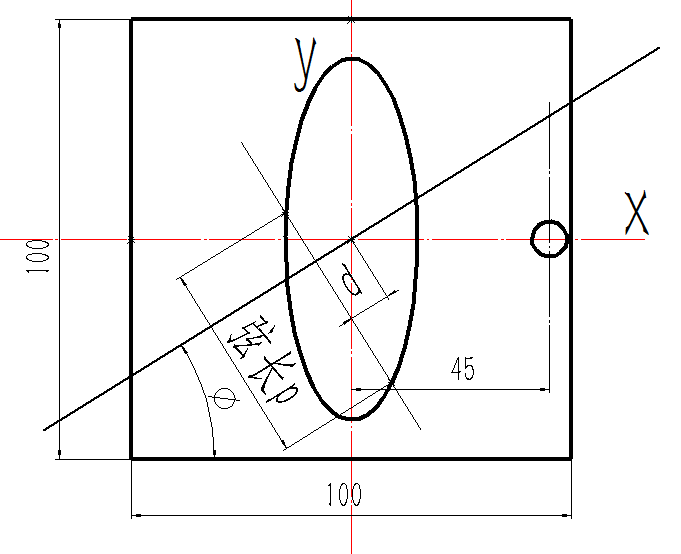
\includegraphics[width=\textwidth]{./pic/q10.png}
		\end{minipage}
		\begin{minipage}[H]{0.45\textwidth}
		\centering
		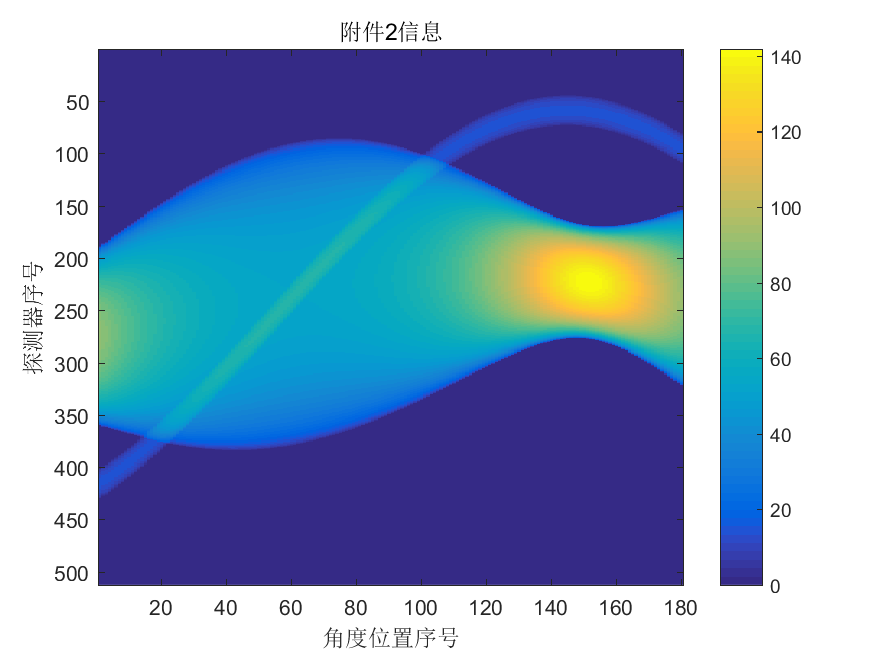
\includegraphics[width=\textwidth]{./pic/fujian2.png}
		\end{minipage}
	\end{figure}

\end{frame}

\begin{frame}{初步计算参数}
	\small 使用最小二乘法对曲线进行拟合,求出各个参数的值为:
	\[\mu =1.7724 , \Delta d = 0.2768, d_0 = -4.0688, c = 0.0000\]
	\begin{figure}[H]
		\centering
		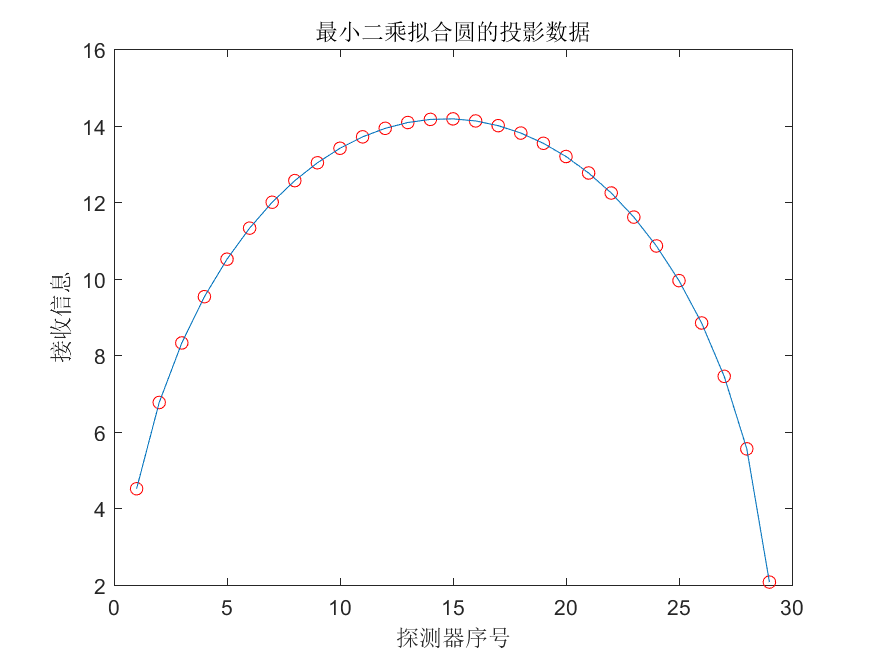
\includegraphics[width=0.8\textwidth]{./pic/fitCir.png}\\
		\caption{拟合圆上的数据}
	  \end{figure}

\end{frame}



\begin{frame}{完整模型建立}
	以正方形托盘的中心为坐标原点,椭圆中心与圆中心的连线方向为\(x\)轴,过坐标原点垂直于\(x\)轴方向为\(y\)轴,建立平面直角坐标系。在这一坐标系中,设CT系统的旋转中心坐标为\(R(x_0,y_0)\),探测器平面与\(x\)轴的夹角为\(\theta\),探测器中心与旋转中心在探测器平面上的投影的距离为\(d_0\)。
	  
\end{frame}



\begin{frame}{参数定义}
	\begin{figure}
		\begin{center}
			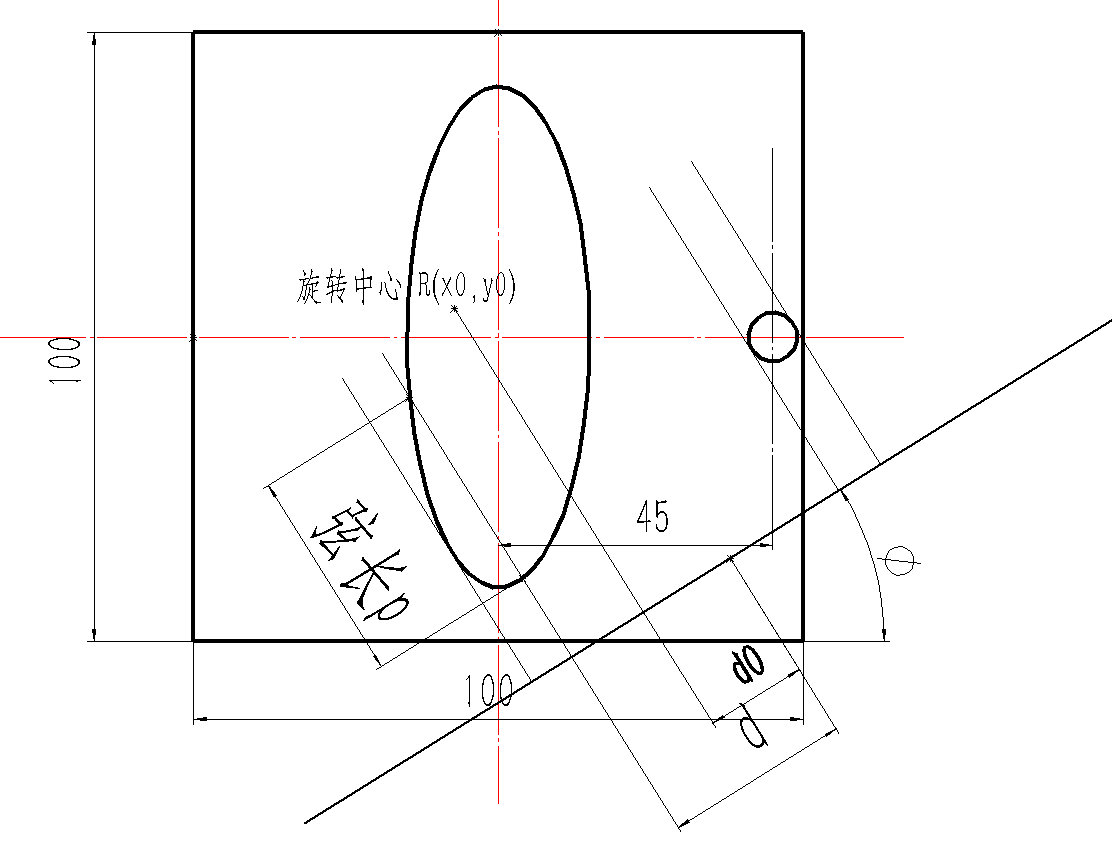
\includegraphics[scale=0.3]{pic/q13.png}
		\end{center}
		\caption{参数定义}
		\label{Fig:xian}
	\end{figure}
\end{frame}



\begin{frame}{求解长度}
	标定模板中,椭圆与圆的方程分别为:
	\[\frac{x^2}{m^2} + \frac{y^2}{n^2} = 1,m = 15,n = 40;(x - 45)^2 + y^2 = 4^2\]
	综合求解,所以对于探测角度为\(\phi\)的探测器,其上第\(i\)条X射线探测所得的数值的计算公式为:
	\begin{tiny}
		\begin{align*}\label{va}
			V = & \mu\frac{2mn\sqrt{\max(0,m^2\cos^2\phi + n^2\sin^2\phi - (x_0\cos\phi + y_0\sin\phi + d_0 +  (i - 256.5)\Delta d)^2})}{ m^2\cos^2\phi + n^2\sin^2\phi} \\
			    & + 2\mu\sqrt{\max(0,r_0^2 - (G\cos\phi - (x_0\cos\phi + y_0\sin\phi + d_0 +  (i - 256.5)\Delta d))^2)}                                                  
		\end{align*}
	\end{tiny}
\end{frame}



\begin{frame}{模型求解}
	\textbf{迭代优化算法}
	\begin{itemize}
		\item 选取参数\(d_0,x_0,y_0,\mu,\Delta d,\phi_i,i=1,\ldots,180\)的初值,这里参数的初值可以随意选取,我们设置为\(d_0 = x_0 = y_0 =  0,\mu = 1.7724\)(由前文初步计算得),使用\(512\times 180\)组数据,对所有参数进行拟合,获得第一次求解的参数结果。
		\item 对第一次求解得到的\(\phi_{1_i},i=1,\ldots,180\),对数据进行平滑处理,接着将\(\phi_i\)作为已知参数,使用\(512\times 180\)组数据,以第一次求解的结果作为初值,对参数\(d_0,x_0,y_0,\mu,\Delta d\)进行求解,得到第二次参数的求解结果。
	\end{itemize}
\end{frame}
% 局部加权回归散点平滑法是什么
% 为什么要平滑


\begin{frame}{模型求解}
	\textbf{迭代优化算法}
	\begin{itemize}
		\item 使用第二次求解得到的参数\(d_0,x_0,y_0,\mu,\Delta d\)作为已知参数,对于180组,每组512个数据,以第(2)步中得到的角度作为初值,分别对每组数据的角度参数进行求解,得到第(3)步的求解结果。
		\item 使用第(2)步与第(3)步的结果作为初始值,再次使用\(512\times 180\)组数据,对所有参数进行拟合,得到最终结果。
	\end{itemize}
	经测试,经过这样几次求解之后,所得值已经稳定,再次求解结果不会有明显改变。
	% 得说明一下继续迭代结果保持稳定
	% 妈的这里好像没法跨页写enumerate
\end{frame}




\begin{frame}{求解结果} 
	\small 使用上述算法对模型进行求解,得到各个参数如下:
	\[\mu = 1.7727,x_0 = -9.2696,y_0 = 6.2738\]
	\[d_0 = 0.0000,\Delta d = 0.2768\]
	\small 根据所建坐标系 ,CT系统X射线逆时针旋转的始值为-60.3465$^\circ$,终值 118.6439$^\circ$。
	\midpic{q12.png}{标定板示意图}
\end{frame}




\section{问题二的求解}

\begin{frame}{求解思路}
	\begin{enumerate}
		\item 预备知识:拉东变换(Radon Transform)
		\item 连续模型——滤波反投影算法(FBP)
		\item 离散模型——代数迭代法(ART)
	\end{enumerate}
	\begin{figure}[H]
		\centering
		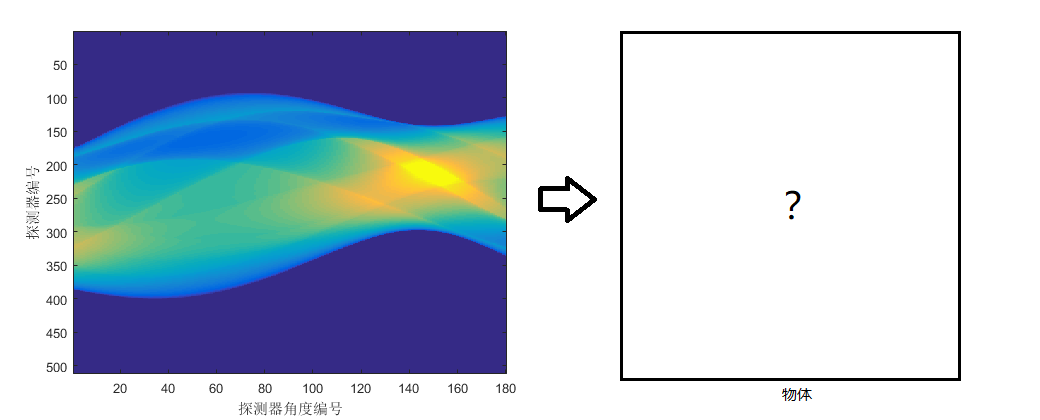
\includegraphics[width=1\textwidth]{./pic/pro3.png}\\
		\end{figure}
\end{frame}



\begin{frame}{数据预处理}
	由问题一可知,由于安装过程的误差,CT系统的旋转中心并不在正方形的中心,由前文推导公式可知,探测器上的第\(i\)个传感器与坐标原点的沿探测器方向的距离为:
	\[d' = x_0\cos\phi + y_0\sin\phi + d_0 +  (i - 256.5)\Delta d\]
	对于任意角度的探测器,我们都可以设置一个中心与原点重合的辅助探测器,将探测器上的数据转化到辅助探测器上,再对问题进行求解。
	即:
	\[d' = (i' - 256.5)\Delta d = x_0\cos\phi + y_0\sin\phi + d_0 +  (i - 256.5)\Delta d\]
\end{frame}



\begin{frame}{数据预处理}
	则对于原始数据\( y = data(i,j)\),可以得到新的转化后的数据
	\[data_{pre}(i',j) = data(i(i'),j)\]
	\[ = data(i' - (x_0\cos\phi + y_0\sin\phi + d_0)/\Delta d,j)\]
	\midpic{datapre3.png}{数据预处理}
\end{frame}



\begin{frame}{连续模型}
	\begin{theorem}	{Fourier Slice Theorem}
		Line Intergal of the Picture
		\[ P_\theta (t) = \int_{(\theta, t) line}f(x, y)\ ds \]
		FT of $P_\theta (t)$
		\[S_\theta (w) = \int_{-\infty}^{\infty}P_\theta (t) e^{-j2\pi wt}dt \]
		Fourier Slice Theorem  
		\[\mathcal{F}\{f(x,y)\}(\omega cos\theta,\omega sin\theta)=\mathcal{F}\{P_\theta(t)\}(\omega)\]
	\end{theorem}
	  
	\footnotesize 傅里叶中心切片定理将\textbf{投影}与\textbf{图像}两者在频域建立了联系。实际情况均为离散化数据,可使用FFT等进行计算;使用滤波反投影法 (FBP) 进行重建。
	  
\end{frame}
  
  
  
\begin{frame}{连续模型:FBP} 
	算法步骤如下:  
	\begin{enumerate}
		\item 指定$\theta$,对\(P_\theta (t)\)应用FFT,得到\(S_\theta (w)\)
		        
		\item 对\(S_\theta (w)\)做滤波,本文使用Ramp函数
		        
		\item 应用iFFT于滤波后的结果,得滤波后的投影矩阵
		        
		\item 对投影矩阵插值,进行反投影,本文使用nearest方式
		%ifft得到的是探测器各单元的值,反投影将这个值“抹”到该单元对应的射线经过的像素上,邻近插值就是为像素找到经过它的射线        
		\item 遍历所有的$\theta$    
	\end{enumerate}
\end{frame}
% Ramp滤波是怎么回事?Ramp就是频谱上三角形滤波器,滤去一些高频信号
% 插值又是个啥,我咋不记得
  
  
\begin{frame}{离散模型}  
	设图片共有\(J = n\times n\)个像素,记$\textbf{x}=[x_{1},x_{2} ,\ldots ,x_{J}]^T$为J维图像矢量,\(x_j\)表示图像上第\(j\)个像素点的吸收强度;$\textbf{p}=[p_{1},p_{2} \ldots p_{I}]^T$为I维投影矢量,$p_i$表示第\(i\)条射线所经过的所有像素的投影值,$R=(r_ij)_{I\times J}$为投影矩阵,\(r_ij\)为0-1变量表示宽为\(\delta\)的粗射线\(i\)是否穿过像素\(j\),则	  
	\begin{equation}
		R\textbf{x}=\textbf{p}
	\end{equation}
\end{frame}
  
  
  
\begin{frame}{离散模型:ART}
	  
	ART(代数迭代法)的思路是每次校正一条射线路径上的像素值,使得该条真伪射线和间误差减小。迭代公式为:ART(代数迭代法)的思路是每次校正一条射线路径上的像素值,使得该条真伪射线和间误差减小。迭代公式为:
	  
	\begin{equation}
		x^{(k+1)}=x^{(k)}+\lambda^{(k)}\frac{p_{i_{k}}-r_{i_{k}}x^{(k)}}{||r_{i_{k}}||^{2}}r_{i_{k}}
	\end{equation}
	  
	式中,k是迭代次数,$k=0,1 \ldots$,$i_{k}=k(modI)+1$;$\lambda^{(k)}$称为松弛参数,本文取$\lambda^{(k)}=0.25$
	  
	\begin{alertblock}{Note}
		  
		迭代过程中每步还可应用像素值非负这一限制
		  
	\end{alertblock}
	  
\end{frame}
  
  
  
\begin{frame}{降噪算法}
	本文使用NLM(非局部均值)降噪方式对图像进行处理。 NLM算法是图像降噪领域非常有效的算法之一,效率较高,实现简单。其思路是对像素的某邻域窗口内的像素灰度值做加权平均,且像素越相似,权重越大。
	  
	\begin{equation}
		NLM(x_{i})=\sum_{j\in N_{i}} w(i,j)x_{j}
	\end{equation}
	其中,\(w(i,j)=\frac{e^{-||x_{V_{i}}-x_{V_{j}}||^2/h^2}}{\sum_{j\in N_{i}}e^{-||x_{V_{i}}-x_{V_{j}}||^2/h^2}}\),$N_{i}$表示像素i的邻域,本文取5*5像素窗口,$x_{V_{i}}$是像素i邻域像素的值构成的矩阵,这里矩阵模的意义是各元素平方和的平方根;$h$控制滤波强度,本文取为0.5
\end{frame}
  
  
  
\begin{frame}{求解结果}
	  
	\small 重建之前,先将数据进行预处理,变换到旋转中心与原点重合且关于过原点的垂线对称的参考探测器上\\
	  
	\begin{figure}[H]
		\begin{minipage}[H]{0.5\textwidth}
		\centering
		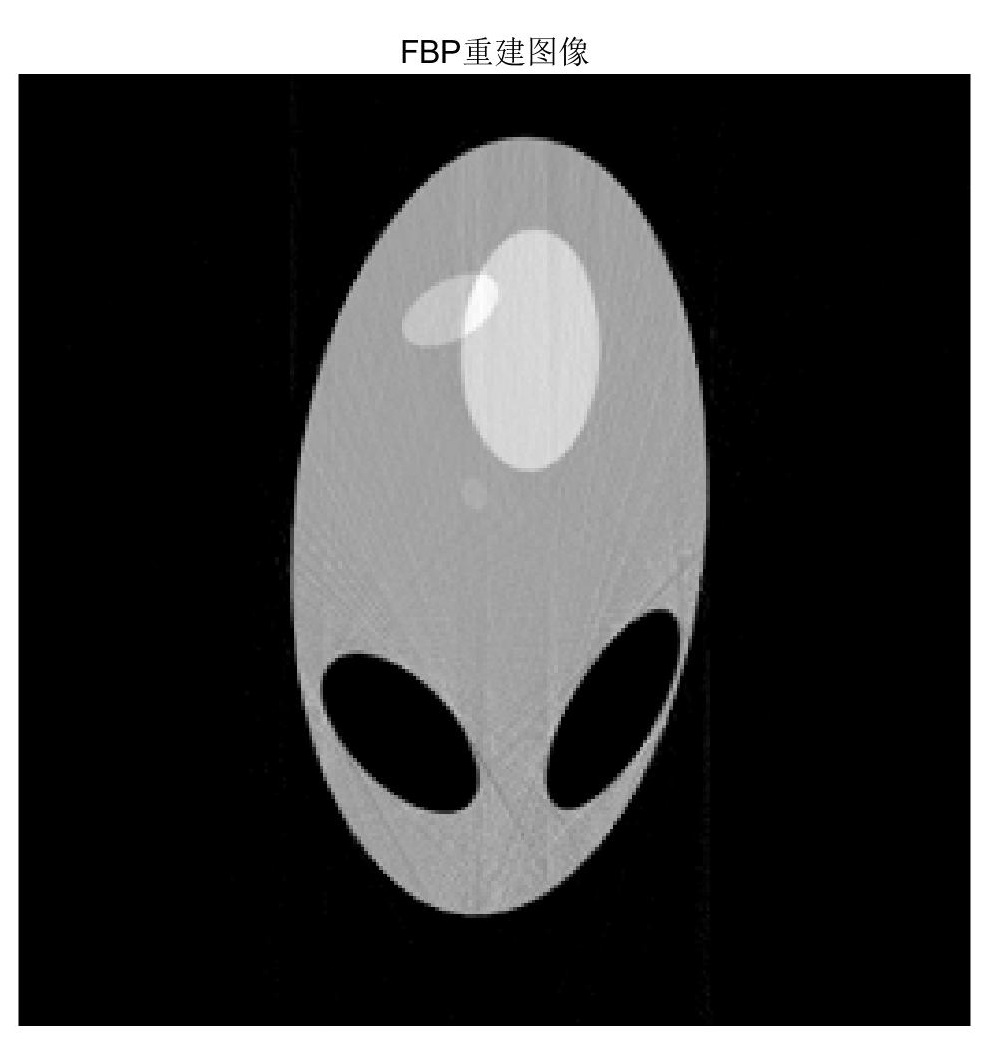
\includegraphics[width=\textwidth]{./pic/P2_FBP.jpg}
		\end{minipage}
		\begin{minipage}[H]{0.5\textwidth}
		\centering
		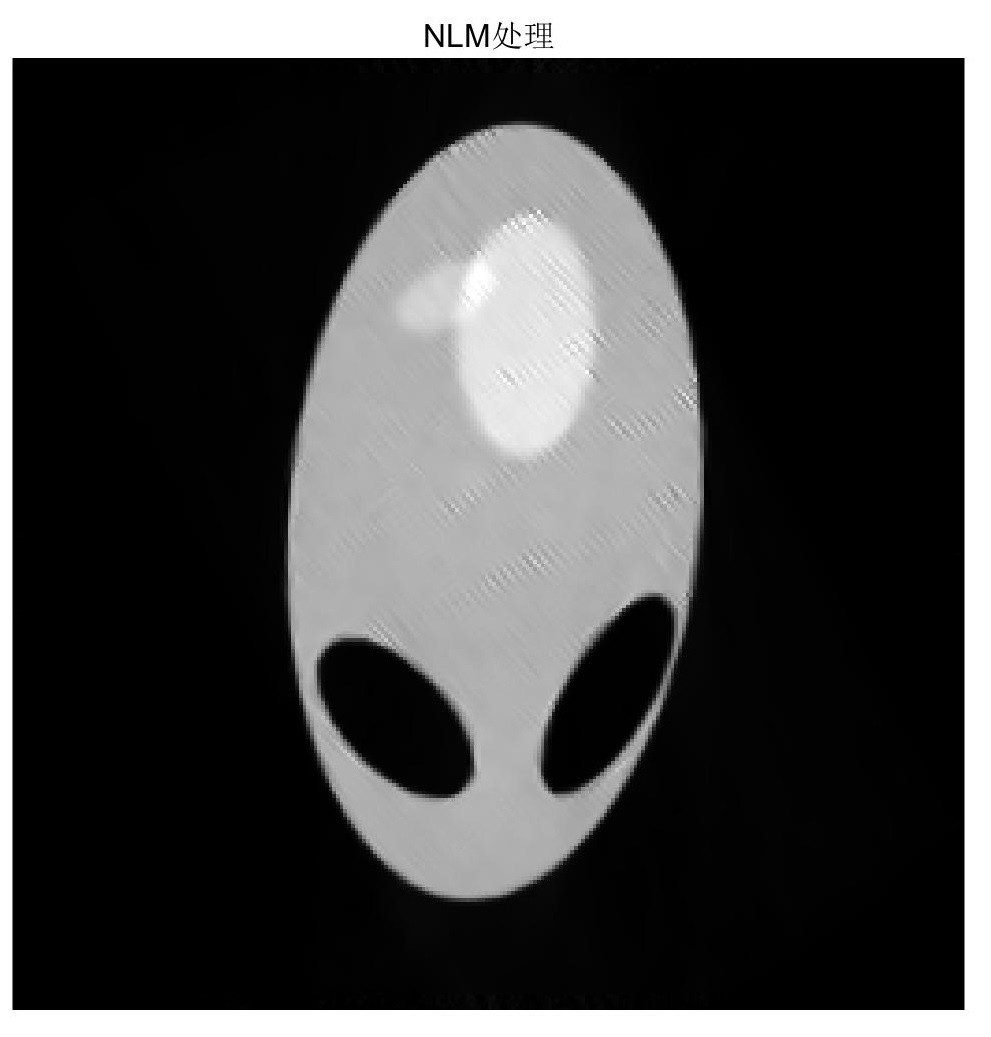
\includegraphics[width=\textwidth]{./pic/P2-ART-5-NLM.jpg}
		\end{minipage}
	\end{figure}
	  
	算法输出结果再做适当的缩放和比例处理即为最终结果。
	  
\end{frame}



\begin{frame}{求解结果}

	\small 以下为指定点处的重建值

	\begin{figure}[H]
		\centering
		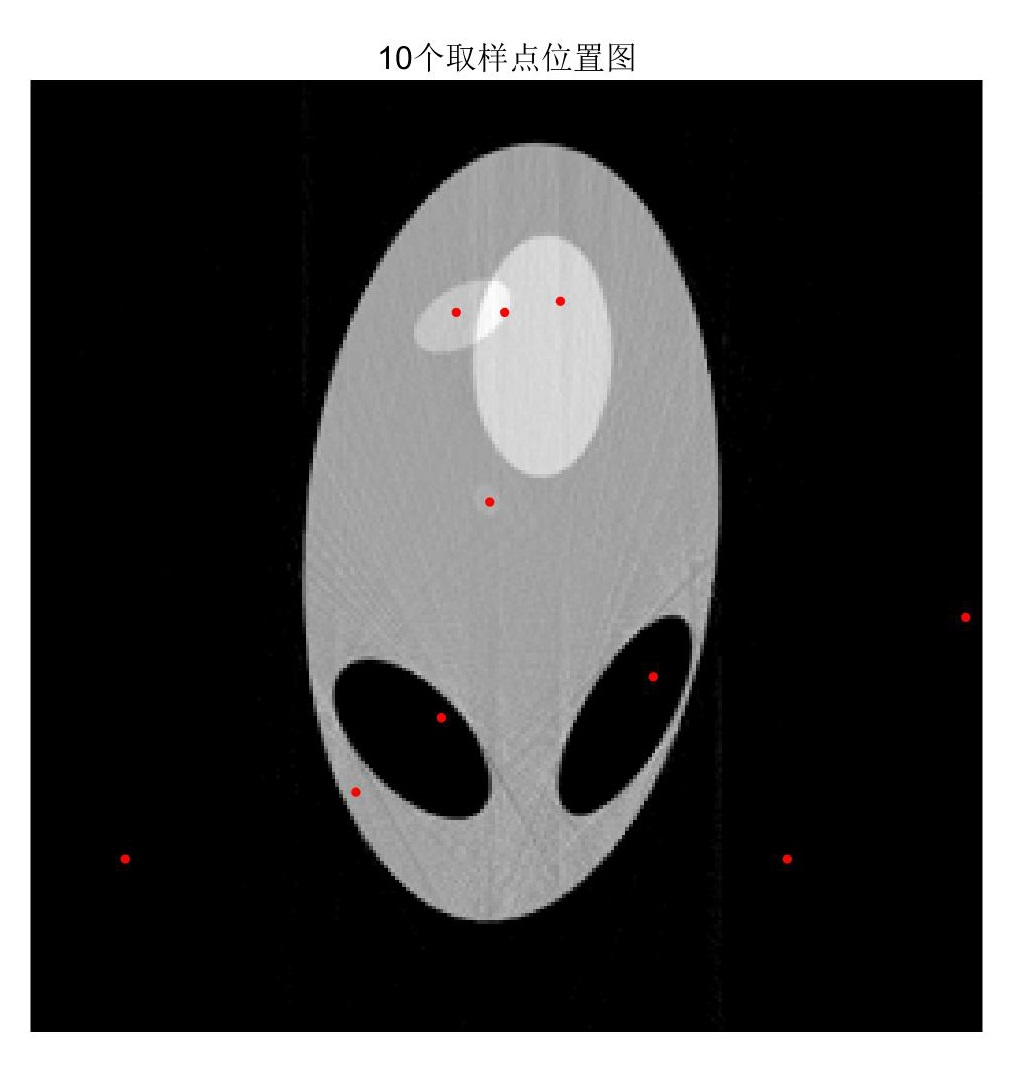
\includegraphics[width=0.3\textwidth]{./pic/DOT.jpg}
	\end{figure}
	
	\begin{table}[H]
		\centering
		\begin{tabular}{ccccccccccc}
			\toprule
			\text{No.}   & 1 & 2 & 3 & 4 & 5 & 6 & 7 & 8 & 9 & 10 \\
			\midrule
			\text{Value} & 0.0070 & 0.6943 & 0.0106 & 0.8269 & 0.7285 & 0.9269 & 0.9111 & 0.0000 & 0.0062 & 0.0000 \\
			\bottomrule
		\end{tabular}
	\end{table}

\end{frame}		



\section{问题三的求解}
  
\begin{frame}{求解思路}
   \begin{figure}[H]
		\begin{minipage}[H]{0.45\textwidth}
		\centering
		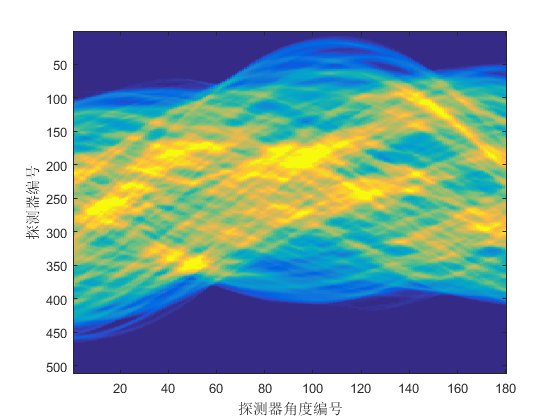
\includegraphics[width=\textwidth]{./pic/fujian5_2.png}
		\end{minipage}
		\begin{minipage}[H]{0.5\textwidth}
		\centering
		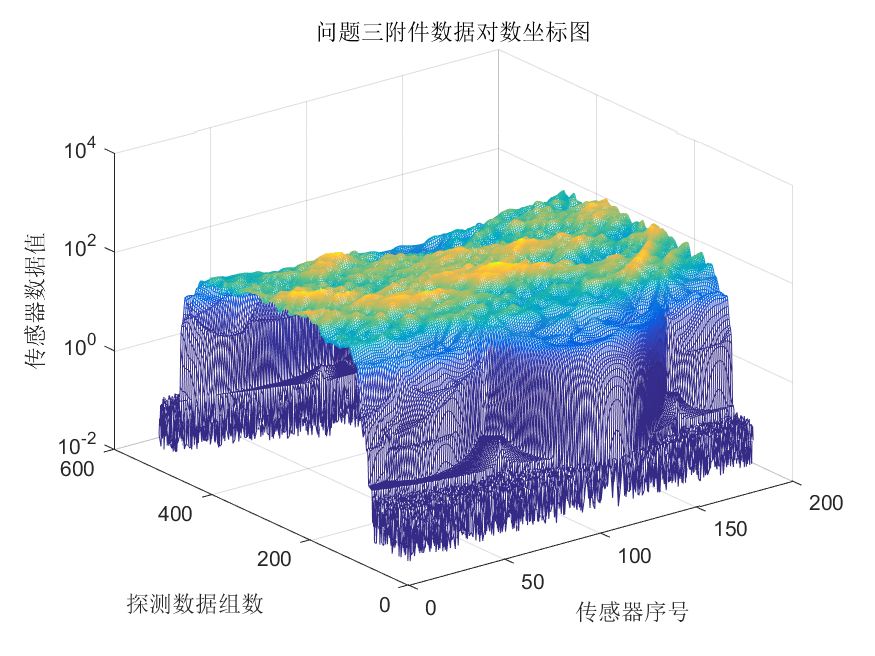
\includegraphics[width=\textwidth]{./pic/fujian5.png}
		\end{minipage}
	\end{figure}
	与第二问区别:增加噪声。数据更复杂,考验算法鲁棒性。
\end{frame}
  
\begin{frame}{去噪预处理}
	\small 观察数据,发现含有较多噪声:
	  
	\begin{itemize}
		  
		\item \small 一方面,作差分图(下图)可见主要数据集中在探测器中间部位,边缘部分值远小于主要数据值
		        
		\item \small 另一方面,绘制对数坐标图可见边缘数值无规律波动
		        
	\end{itemize}
	  
	同时,根据对数坐标图,考虑噪声水平约为0.3,筛选小于0.3的值进行进一步检验。画出分布直方图,猜想其近似服从均为分布;利用SPSS做Kolmogorov-Smirnov均匀分布检验。
	
	\begin{figure}[H]
		\centering
		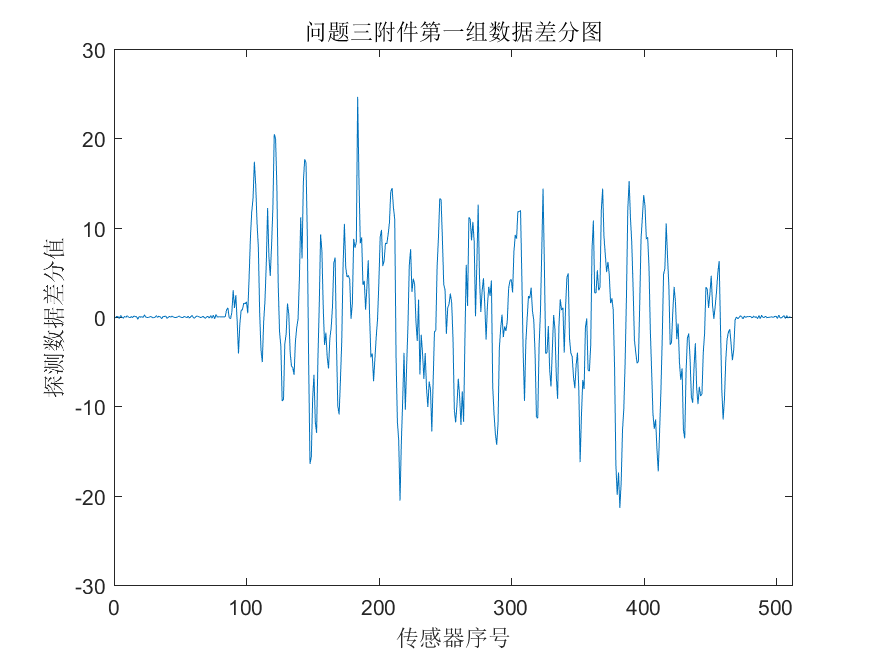
\includegraphics[width=0.5\textwidth]{./pic/fujian5_1.png}\\
	\end{figure}
\end{frame}
  
  
  
\begin{frame}{去噪预处理}
	  

	\small 探测器两边的相邻两个传感器的数据差集中在0 附近,因此我们推测这些数据是由测量时的误差引起的波动。
	  
	\small 检验结果接受原假设(均匀分布),均值为0.1549,显著性水平0.157\\
	\begin{figure}[H]
		\centering
		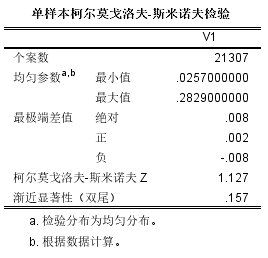
\includegraphics[width=0.5\textwidth]{./pic/K-S.jpg}\\
	\end{figure}
	\small 因此,对原数据做去噪处理,本文将非主信号区域的噪声删去并在主要信号值上减去噪声均值。之后再按照问题二所述方法进行预处理,并分别使用ART算法与FBP算法进行重建。
	  
\end{frame}
  
  
  
\begin{frame}{求解结果}
	\begin{figure}[H]
		\centering
		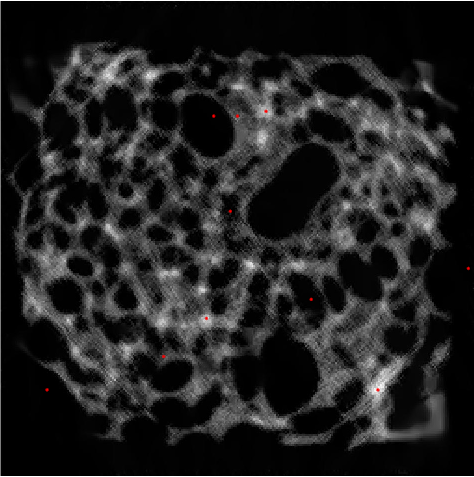
\includegraphics[width=0.3\textwidth]{./pic/res3.png}\\
	\end{figure}

	\begin{table}[H]
		\centering
		\begin{tabular}{ccccccccccc}
			\toprule
			\text{No.}   & 1 & 2 & 3 & 4 & 5 & 6 & 7 & 8 & 9 & 10 \\
			\midrule
			\text{Value} & 0.0212 & 3.5766 & 8.5109 & 0.0136 & 0.0349 & 3.8526 & 8.1648 & 0.0413 & 7.9565 & 0.0051 \\
			\bottomrule
		\end{tabular}
	\end{table}

	\small 依然,使用FBP求解结果较小。ART更加精确。
\end{frame}
  
  
  
\begin{frame}{对比与评价}
	  
	对比两种算法,ART-NLM算法的重建速度较慢,成像质量略差与FBP。我们认为这是由于投影矩阵$R$元素为0-1变量造成的;每次做迭代修正时,射线边缘的像素也同时受到等值的修正,造成了一定的偏差\\
	  
\end{frame}



\section{问题四的求解}

\begin{frame}{精度分析}
	在这个问题中,我们采用模拟仿真的方法进行精度分析。在问题一模型的基础上,我们通过更改位置参数信息,进行模拟,得到这种情况下的\(512\times180\)个数据,再使用我们的模型,在这组数据的基础上进行标定,计算得出标定所需参数,与设定的理论值进行对比,即可得到模型的精度信息。
\end{frame}

\begin{frame}{精度分析}
	设置参数\(d_0 = 1,\mu = 1.5,x_0 = 10,y_0 = 10\),观测角度依次为\(\phi_i = i^\circ,i = 1,\ldots,180\),使用问题一中模型,模拟生成180组探测器数据。将生成的探测器数据进行参数标定,得到结果如表\ref{jingdu}所示。 
	\begin{table}[H]
		\centering
		\caption{计算机仿真实验的几何标定结果}
		\label{jingdu}
		\begin{tabular}{ccccc}
			\toprule 
			\text{参数名称}               & \(d_0(mm)\) & \(x_0(mm)\) & \(y_0(mm)\) & \(\mu\) \\
			\midrule 
			\text{理论值}                  & 5           & -8          & 10          & 1.5     \\
			\text{计算值}                  & 5.0000      & -8.0000     & 10.0000     & 1.5000  \\
			\text{差值}(\(\times10^{-10}\)) & -0.1195     & -0.0022     & -0.5961     & -0.0135 \\
			\bottomrule
		\end{tabular}
	\end{table}
\end{frame}

\begin{frame}{稳定性分析}
	使用计算机进行仿真,人为地在投影坐标中增加不同等级的噪声数据,再以此进行模板标定。
	与精度分析相同,设置参数\(d_0 = 1,\mu = 1.5,x_0 = 10,y_0 = 10\),观测角度依次为\(\phi_i = i^\circ,i = 1,\ldots,180\),使用(1)中模型,模拟生成180组探测器数据。根据这种方法模拟得到的探测器接受信息中的数据范围在(0,120)之间,我们给原数据增加在(-15,15)范围内均匀分布的随机噪声。从数据图中可以看出,数据信息较原数据更模糊,且噪声较多。

	\begin{alertblock}{Note}
		\small 这里有一个问题就是实际的探测器数值是不会有负值的,我们在做的时候没有考虑到这一点,导致生成的探测器数据会有负值。
	\end{alertblock}
\end{frame}

\begin{frame}{稳定性分析}
	\doublepic{zaoyin2.png}{投影数据}{zaoyin30_wucha.png}{角度计算误差}
	角度计算的均方根误差为0.0053rad,结合图像与表格数据,我们可以看出,我们的标定算法在数据有小范围的噪音的时候,标定产生的误差仍然较小,算法具有很好的稳定性。
\end{frame}

\begin{frame}{稳定性分析}
	\doublepic{zaoyin3.png}{(-50,50)噪声的投影数据}{zaoyin50_wucha.png}{角度计算误差}
\end{frame}

\begin{frame}{稳定性分析}
	\begin{table}[H]
		\centering
		\caption{(-50,50)均匀分布的噪声误差}
		\label{50zao}
		\begin{tabular}{ccccc}
			\toprule 
			\text{参数名称} & \(d_0(mm)\) & \(x_0(mm)\) & \(y_0(mm)\) & \(\mu\) \\
			\midrule 
			\text{理论值}    & 5           & -8          & 10          & 1.5     \\
			\text{计算值}    & 5.0693      & -8.0188     & 10.3614     & 1.4938  \\
			\text{差值}       & -0.0693     & 0.0188      & -0.3614     & 0.0062  \\
			\bottomrule
		\end{tabular}
	\end{table}
	角度计算的均方根误差为0.0191rad,相比噪声较小时,参数标定的误差有所增大,但仍然在很小的范围内。
\end{frame}

\begin{frame}{新标定模板的设计}
	为何设计新模板?
	\begin{itemize}
		\item 模板易于加工。
		\item 模板中的特征图形可以写出简洁的解析表达式。
	  \end{itemize}
	在第一问中,我们未使用特殊的几何特征点,直接利用数据求解。在自行设计模板中,考虑使用几何信息来推算标定参数的初值。
\end{frame}

\begin{frame}{新标定模板的设计}
	\doublepic{sketch1.png}{新标定模板的示意图}{sketch2.png}{几何关系示意图}
	有对称信息,但不中心对称。几何形状简单,便于寻找特殊点。
\end{frame}

\begin{frame}{新标定模板的设计}
	\begin{figure}[H]
		\centering
		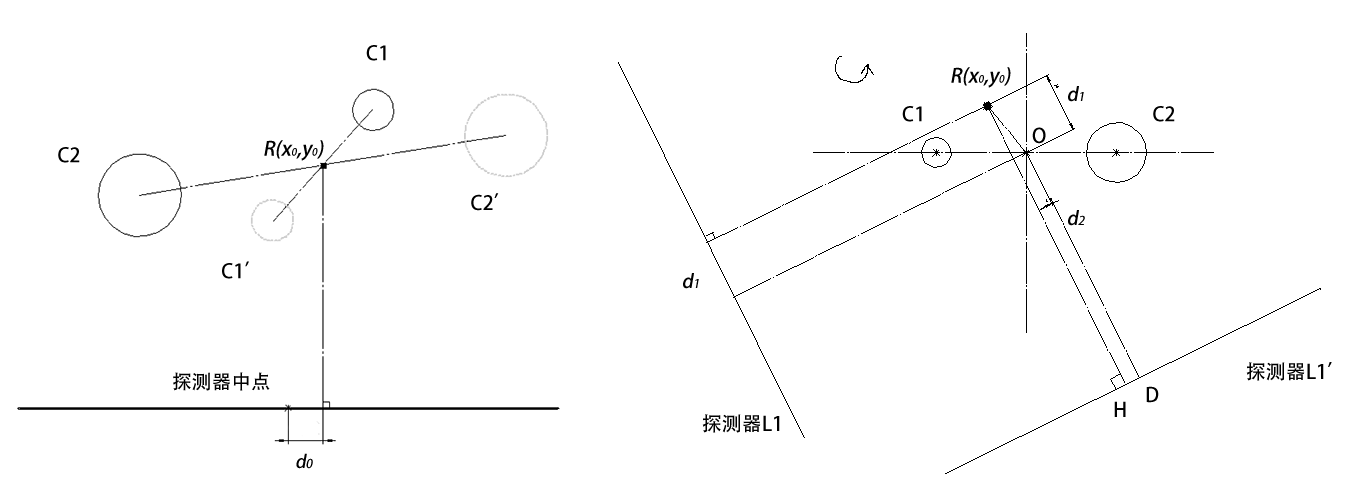
\includegraphics[width=\textwidth]{./pic/merge1.png}\\
	\end{figure}
	\small 根据第1个角度和第180个角度时两个圆的投影相对位置,得圆心坐标:
	\[ i_R = \frac{i_1 + i_2 + i_1' + i_2'}{4} \]
	\[d_0 = (256.5 - i_R) \times \Delta d\]
	
\end{frame}

\begin{frame}{新标定模板的设计}
	\begin{figure}[H]
		\centering
		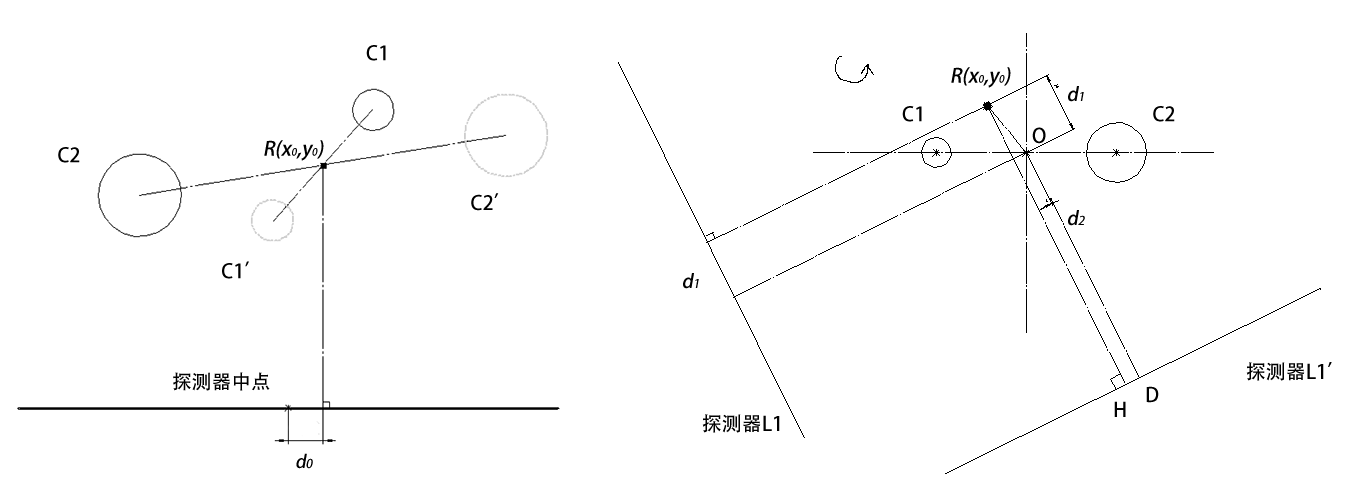
\includegraphics[width=\textwidth]{./pic/merge1.png}\\
	\end{figure}
	\small 当前探测器与\(x\)轴的夹角\(\phi\)的估计值为:
	\[ \phi = arcsin\left(  \frac{(R1_{c1} - R2_{c1})\Delta d}{C_1 C_2}   \right)\]
	\small 再考察第90组CT观测数据,此时探测器相对于初始位置逆时针旋转了大约90°。\(\angle ROD = arctan(HD/H'D') \),\(OR\)与\(x\)轴的夹角为 \( \theta _R = \phi + \pi/2 - \angle ROD \),则\(R\)坐标为:
	\[x_0 = |OR| \times cos(\theta_R), y_0 = |OR| \times sin(\theta_R) \]
	
\end{frame}

\begin{frame}{新标定模板的使用评价}
	\midpic{Error.png}{\(x_0\)相对误差示意图}
	\small 可见60\% 的角度中,\(x_0\)的相对误差小于0.5\%,误差为取最大值3.78\%。经分析,误差偏高的原因为解非线性规划时陷入局部最优解。这时用得到的解作为初始值,使用模拟退火算法继续求解,可以将最终的相对误差缩小到0.13\%。
	\small 与第一问中的算法相比,本模板只进行\textbf{一次}迭代优化即可得到精度较高的结果,计算量相对较小。
\end{frame}


\section{改进与讨论}

%下面这个part有bug,暂时还没找到
% \begin{frame}{\textbf{ART(代数迭代法)的改进}}
% 	\small 重新定义\textbf{投影矩阵}:设图片共有\(J = n\times n\)个像素,共有$I$条射线进行扫描,$R=(r_{ij})_{I\times J}$,其中$r_ij$表示射线$i$与像素$j$相交的线段长度

% 	\textbf{原方法:}构造256$\times$256的矩阵$r$,令其中一列等于1,旋转$r$,得到投影值。
% 	\textbf{新方法:}
% 	\begin{itemize}
% 		\item 写出直线方程
% 		\item 求出指定行与直线相交最左与最右的像素
% 		\item 顺序计算上述范围内每个像素的$r$值
% 		\item 遍历所有的行
% 	\end{itemize}

% 	\begin{table}[H]
% 		\caption{改进后的第三问重建结果}
% 		\centering
% 		\begin{tabular}{ccccccccccc}
% 			\toprule
% 			\text{No.}   & 1 & 2 & 3 & 4 & 5 & 6 & 7 & 8 & 9 & 10 \\
% 			\midrule
% 			\text{Value} & 0.0212 & 2.8719 & 7.0425 & 0.0136 & 0.0349 & 3.2979 & 6.2002 & 0.0413 & 7.8576 & 0.0051 \\
% 			\text{Value_F} & 0.0192 & 2.8713 & 7.0418 & 0.0133 & 0.0339 & 3.2973 & 6.1999 & 0.0408 & 7.8566 & 0.0049 \\
% 			\text{Value_R} & 0.0063 & 2.5658 & 6.8698 & 0.0076 & 0.0185 & 3.3793 & 6.2005 & 0.0025 & 8.2590 & 0.0071 \\
% 			\bottomrule
% 		\end{tabular}
% 	\end{table}
% \end{frame}

\begin{frame}
	\begin{itemize}
		\item \textbf{FBP(滤波反投影)的讨论}
	\end{itemize}

	\small FBP中反投影矩阵的维度一定为探测单元数,即512。实际图像中存在将结果resize为256*256的过程,在其中需要乘以一个系数;同时在缩放过程中,像素的值也需要做调整\\
	\small 另一方面,因为在连续模型中使用FFT会导致舍入误差的出现,加上FBP中有一个低通滤波,会使数据有一定失真,导致FBP的结果比实际结果要小。
\end{frame}

\section{参考文献}
\begin{frame}{参考文献}
	\begin{thebibliography}{0}
		\bibitem{toumo}
		Kak A C. BOOKS AND PUBLICATIONS:"Principles of Computerized Tomographic Imaging"[J]. Medical Physics, 2002, 29(1):107.
		    
		\bibitem{nlm}
		J. Huang et al, "Sparse angular CT reconstruction using non-local means based iterative-correction POCS," Computers in Biology and Medicine, vol. 41, (4), pp. 195-205, 2011.
		    
		\bibitem{ct1}庄天戈. CT原理与算法[M]. 上海交通大学出版社, 1992.
		\bibitem{radon}林世明, W.-M.Boerner. 离散Radon变换[J]. 西北工业大学学报, 1988(2):49-56.
	\end{thebibliography}
\end{frame} % 



\section{心得与体会}
\begin{frame}{赛前}
	\begin{enumerate}
	  \item 五月六月,总结得失,制定计划。
		\begin{enumerate}
		  \item[-] 比赛四天,规划好时间
		  \item[-] 留出充足时间写论文
		\end{enumerate}
	  \item 八月九月,准备国赛,扩充知识。
		\begin{enumerate}
		  \item[-] 最优化求解算法——SA, GA, NN, etc.
		  \item[-] 数值计算——Runge-Kutta, Simpson, Gauss, etc
		  \item[-] 模型建立——\emph{Optimization Model with LINGO}, 往届国赛题
		  \item[-] 一定要有书面笔记,给自己和队友交代
		\end{enumerate}
	  \item 赛前一定要制定好比赛期间的时间轴!
	\end{enumerate}
\end{frame}

\begin{frame}{我们的比赛时间轴}
	\begin{enumerate}
	  \item \small 9月14日20:00发题,24:00前确定题目,把整个题目框架搭好。
	  \item \small 9月15日中午之前,第一问模型建立,开始求解。
	  \item \small 9月15日20:00前把第一问结束。开始着手第二三问,建立二三问模型。
	  \item \small 9月16日中午之前,第二问第三问模型基本建成,开始求解。同时着手稳定性分析。抽空思考自己设计的模板。
	  \item \small 9月16日下午开始写论文,把能写的先写掉。
	  \item \small 9月16日24:00前把第二问和第三问解决。
	  \item \small 9月17日写论文,完善模型及求解,完成第四问。
	\end{enumerate}
	\begin{center}
	  \textbf{总体先紧后松,留充足时间推敲论文,微调模型。}
	  
	  \textbf{计划赶不上变化,但一定要预留充足时间。}
	\end{center}
\end{frame}

\begin{frame}{MATLAB创新奖}
	\begin{enumerate}
	  \item \small 原创算法——标定,FBP,ART。
	  \item \small 只使用数据,不考虑几何特殊点——基于丰富的求解经验。
	  \item \small 准确发现第三问与第二问的区别——加均匀分布噪声。
	  \item \small 论文框架完整——第一到四问模型+稳定性分析+模型评价。
	\end{enumerate}
	\small MATLAB中有自带解决该问题的函数iradon.m,我们是五个优秀论文组中唯一没用该函数的队伍;同时我们是五个优秀论文组分析了数据噪声水平的队伍。
\end{frame}

\begin{frame}{MATLAB程序的有趣之处}
	%% TODO: 研究一下其他组的第一问
	%woc bug在哪里啊!!!!
	% \begin{table}[H]
	% 	\centering
	% 	\caption{优秀论文第一问解法对比}
	% 	\begin{tabular}{ccccc}
	% 		\text{No.} & A156 & A298 & A053 & A090\\
	% 		$\Delta$ & \text{几何特征+搜索} & \text{几何特征} & ? & ? \\
	% 		\text{d_0} & \text{未解} & \text{未解} & ? & ? \\
	% 		\text{(x_0,y_0)} & \text{几何特征+搜索} & \text{几何特征} & ? & ? \\
	% 		$\mu$ & \text{小圆平均} & \text{特征位置} & ? & ? \\
	% 		$\theta$ & \text{遍历搜索} & \text{非线性优化} & ?& ?\\
	% 	\end{tabular}
	% \end{table}

\end{frame}


\bibliographystyle{IEEEtran} % comment this line if nothing is cited
\bibliography{bibliography_file} % comment this line if nothing is cited

%\end{CJK*}
\end{document}

% \label{Sec:model}
% \begin{frame}{2. Mathematical model 数学模型}
% 	Lists 列表
	
% 	\begin{description}
% 		\item[Description list] is a type of list to describe items.
% 		\item[Description list] 是一种用于描述的列表。
% 	\end{description}
% \end{frame} 
% \begin{frame}{1. Introduction 引言}
% 	\framesubtitle{frame subtitle 页面副标题}
% 	This nuaa-JUB.tex is a \LaTeX \ Beamer template using the JUB Beamer theme  produced by Billy Okal.
	
% 	\bigskip
	
% 	此nuaa-JUB.tex文件是一个使用了Billy Okal制作的JUB Beam主题的\LaTeX \ Beamer模板。
	
% 	\begin{figure}
% 		\begin{center}
% 			
\includegraphics[scale=0.1]{latex.png}
% 		\end{center}
% 		\caption{\LaTeX \ beamer}
% 		\label{Fig:latex_beamer}
% 	\end{figure}
% \end{frame} % 
% \section{Empirical experiments}
% \label{Sec:experiments}
% \begin{frame}{3. Empirical experiments 实验}
% 	Blocks 区块
	
% 	\begin{definition}[Pythagorean theorem]
% 		The Pythagorean theorem is a fundamental relation in Euclidean geometry among the three sides of a right triangle.
% 	\end{definition}
	
% 	\begin{theorem}[Pythagorean theorem]
% 		$a^2 + b^2 = c^2$
% 	\end{theorem}
% \end{frame} 

% \begin{frame}{3. Empirical experiments 实验}
% 	Blocks 区块
	
% 	\begin{exampleblock}{For example}
% 		$3^2 + 4^2 = 5^2$
% 	\end{exampleblock}
	
% 	\begin{alertblock}{Note}
% 		Note that the Pythagorean theorem can only be applied to right triangles.
% 	\end{alertblock}
% \end{frame} 

% \begin{frame}
% 	\begin{center}
% 		\Huge{\bf{Thank you!}}
% 	\end{center}
% \end{frame} 
% ================================================================